\documentclass[a4paper,11pt]{article}
\newcommand\tab[1][0.6cm]{\hspace*{#1}}
\usepackage{mlsubmit}
\usepackage{amsmath}
\begin{document}

\title{MATH578A Assignment 1 }
\author{Raktim Mitra \\ \small{USC ID: 1487079265\hspace{10pt} email: raktimmi@usc.edu}}
\maketitle
\initmlsubmision{1}                              					% assignment number
								{Raktim Mitra}      						           		% your name
								{150562}																		% your roll number
								
\section*{Q1. }

\begin{center}
 -------------------
\end{center}

\section*{Q2. (Chapter 1, exercise 11)}
\textbf{Q}: Let T be a text string of length m and let S be a multiset of n characters. The problem is
to find all substrings in T of length n that are formed by the characters of S. For example,
let S = \{a, a, b, c\} and T = `abahgcabah'. Then `caba' is a substring of T formed from the
characters of 5.
Give a solution to this problem that runs in O(m) time. The method should also be able to
state, for each position i, the length of the longest substring in T starting at i that can be
formed from S.
\\
\textbf{Ans}: Let, A[ ] contains unique elements of S. Count[ ] array contains number of occurences of each element of A in S.


Now, we shall construct the array D[ ] where D[i] contains length of the longest substring of T that \underbar{ends} at position i which can be formed by elements from S.

i ranges from 0 to m-1. 

We also need a RunningCount[ ] array similar to Count[ ], which will use to keep track of counts of elements of S faced for D[i].

A, Count, RunningCount all have the length count(unique(S)).
Note: A.index[c] gives position of char c in A, constant time since A is of constant length assuming alphabet size is constant. 
Therefore, we can write the following recurrence for D[i].
\[D[i] = \begin{cases}
          0 \text{ if T[i] is not in A (case 1)} \\
          \text{ if T[i] is in A }\begin{cases}
          D[i-1] + 1 &\text{ if RunningCount[A.index[T[i]]] $<$ Count[A.index[T[i]]]} \\&\text{($\uparrow$ case 2a)} \\
          i - j &\text{ if RunningCount[A.index[T[i]]] $==$ Count[A.index[T[i]]] }\\
          &\text{where j is the first occurence of T[i] after i - 1 - D[i-1] }\\&\text{($\uparrow$ case 2b)} \\
          \end{cases} \\ 
         \end{cases}
         \]
For the above recurrence to work properly , we need to update RunningCount in the following manner:
\[\begin{cases}
            \text{ (case 1) RunningCount[i] = 0 for all i  } \\
          \begin{cases}
           \text{ (case 2a) RunningCount[A.index[T[i]]] += 1} \\
          \text{ (case2b)  RunningCount[A.index[T[k]]] $-$= 1, for k in interval (i,j) }\\
          
          \end{cases} \\ 
         \end{cases}
         \] \\
         
After we fill up the array D we can report all starting occurence position as: \{i - size(S) for  i if D[i] == size(S)\}.

We can also construct length of longest substrings \underbar{starting} at i and formed by elements of S from D. Let, this array be B[ ]. Shown in full pseudocode below:

\begin{mlalgorithm}[0.9\textwidth]{H}{Multiset Matching }\vskip-2ex
	\label{algo:tk-means}
	\begin{algorithmic}[1]
		\REQUIRE Text T and Multiset S
		\STATE A $\leftarrow$ Unique(S)
		\STATE initialize Count[0...length(A)] to all 0
        \STATE initialize RunningCount[0...length(A)] to all 0
		\FOR{element e in S}
		\STATE  Count[A.index[e]]++
		\ENDFOR 
		\STATE intiailize D[0...m-1]
		\STATE D[-1] $\leftarrow$ 0 \COMMENT{For convenience, In actual implementation we would hardcode D[0] and start the following loop at 1.}
		\FOR{\{i=0; i $<$ m; i++\}}
            \IF [Case 1]{T[i] not in A } 
            \STATE D[i] $\leftarrow$ 0 
            \STATE \{RunningCount[j] $\leftarrow$ 0 for j in interval [0,length(a))\}
            \ELSIF{RunningCount[A.index[T[i]] $<$ Count[A.index[T[i]]]\COMMENT{Case 2a}} 
            \STATE D[i] $\leftarrow$ D[i-1] + 1 
            \STATE RunningCount[A.index[T[i]]++
            \ELSE [Case 2b]
            \STATE j $\leftarrow$ i - D[i-1] + 1 //Case 2b
            \WHILE{j$\leq$i and T[j] != T[i]}
            \STATE RunningCount[A.index[T[j]]]$--$
            \ENDWHILE
            \STATE D[i] $\leftarrow$ i $-$ j
            \ENDIF
		\ENDFOR
		\STATE Initialize B[0..m-1] \COMMENT{length of substrings longest substrings formed by elements of S from starting positions.}
		\STATE  i $\leftarrow$ 0
		\STATE  Initialize R \COMMENT{List of starting positions of occurences}
		\WHILE[O(m), only correct when i goes from 0 to m-1, the descending order of traversal won't work.]{\{i $<$ m\}} 
            \STATE B[i - D[i]] $\leftarrow$ D[i]
            \IF{D[i] == size(S)}
            \STATE R.add(i - D[i])
            \STATE i++
            \ENDIF
        \ENDWHILE
		\RETURN R, B
	\end{algorithmic}
\end{mlalgorithm}

\textbf{Time Complexity:} Clearly all the preprocessing can be done in O(m) time and so is generating R and B from D.

That leaves constructing D. The for loop (line 9-23) runs m times. Case 1 and Case 2a are clearly O(1) [Assuming alphabet size is O(1)]. However, the while loop (Case 2b, line 18-20) can be O(size(S)) in worst case. 
But, we can use amortized analysis to show that amortized cost of each iteration of the for loop is O(1). The reason is, case2b can decrement RunningCount (line 19) size(S) times only when Case(2a) has been executed size(S) times. (Because only Case 2a increments RunningCount (line 15).)

Therefore, Case 2b can be O(size(S)) only after O(size(s)) iterations of case 2b which are all O(1) iterations. Therefore, on average each iteration takes O(1), making the whole for loop O(m).

Hence, time complexity of Multiset Matching is O(m).
\begin{center}
 -------------------
\end{center}
\section*{Q3. (Chapter 6, exercise 1.)}
\textbf{Q}: Construct an infinite family of strings over a fixed alphabet, where the total length of the
edge-labels on their suffix trees grows faster than O(m) (m is the length of the string). That
is, show that linear-time suffix tree algorithms would be impossible if edge-labels were
written explicitly on the edges.
\\
\textbf{Ans}: Let, $B^k = BBB...B$ ($k$ times)
Then the following  family of strings over the alphabet $\Sigma = \{A,B\}$ is a required example. 
\begin{align*}
 S_n  &= AB^0AAB^1AAB^2A...AB^nA \\
 S_0 &= AA\\
 S_1 &= AAABA\\
 S_2 &= AAABAABBA\\
\end{align*}
Note: $S_n$ has length $(2 + 3 + 4 + ... + (n+2)) = \frac{(n+2)(n+3)}{2}-1 = O(n^2)$.\\Suffix trees for $S_0,S_1, S_2$:
\begin{figure}[H]

\centering
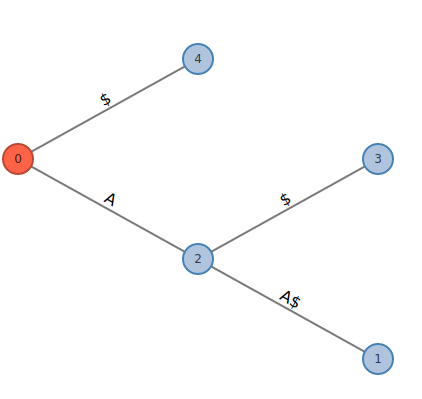
\includegraphics[width=.3\textwidth]{AA.png}\hfill
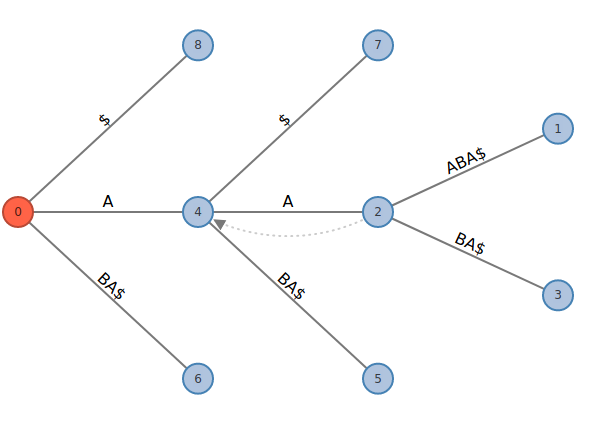
\includegraphics[width=.3\textwidth]{AAABA.png}\hfill
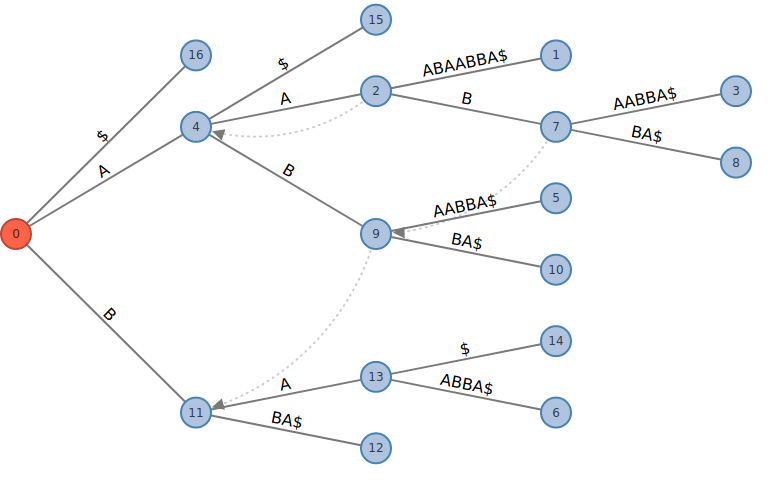
\includegraphics[width=.3\textwidth]{AAABAABBA.png}

\caption{suffix trees for AA, AAABA and AAABAABBA}

\label{fig:figure3}
\end{figure}
We can simply look at how total length of edge labels scales w.r.t lengths of $S_n$:
\begin{center}
\begin{tabular}{ | c | c | c | }
\hline
$n$ & length($S_n$) & total edge label length(excluding \$s) \\ 
\hline
\hline
 0 & 2 & 2\\
 \hline
 1 & 5 & 11 \\  
 \hline
 2 & 9 & 33 \\   
\hline
 \end{tabular}
\end{center}
Clearly total length of edge labels grows much faster than length of the strings.
\begin{center}
 ------------------
\end{center}
\section*{Q4. (Chapter 7, exercise 1.)}
\textbf{Q}: Given a set S of k strings, we want to find every string in S that is a substring of some other string in S. Assuming that the total length of all the strings is n, give an O(n)-time algorithm to solve this problem. 
\\
\\
\textbf{Ans}: We can build a suffix tree in linear time and check if there's an inner node that corresponds to a full string (constant time per node).

Assume we are given strings $S_1,S_2...,S_k$

Build a generalized suffix tree of $S_1\$_1S_2\$_2...S_k\$_k$ with k distinct terminal markers $\$_1,...,\$_k \notin \Sigma$.   

This can be done in linear time.

Assuming that we label leaves with (i,j) if they represent suffix $S_i[j..|S_i|]$ of $S_i$, traverse the tree and find those 𝑛 leaves labelled (i,0), i.e. the leaves that correspond to the full strings.

This takes time linear in the tree size, which itself is linear in the input size.

The descendant leaves of the parent of (i,0) (which is reached by an edge labelled $\$_i$) represent all matches from the set; this follows from the basic invariant of suffix trees. Find any one match by descending to any leaf (but (i,0)).

This again takes linear time.


\begin{center}
-----------------\\
\end{center}

\section*{Q5. (Chapter 7, exercise 2.)}
\textbf{Q}: For a string S of length n, show how to compute the N(i), L(i), L'(i) and sp, values (discussed in Sections 2.2.4 and 2.3.2) in O(n) time directly from a suffix tree for S.
\\
\\
\textbf{Ans}:

\begin{center}

 ------------------ -----------------
\end{center}

\end{document}
